\documentclass[letterpaper,10pt]{article}

\usepackage{enumitem}
\usepackage{titling}
\usepackage{listings}
\usepackage{url}
\usepackage{hyperref}
\usepackage{setspace}
\usepackage{subfig}
\usepackage{sectsty}
\usepackage{pdfpages}
\usepackage{colortbl}
\usepackage{multirow}
\usepackage{multicol}
\usepackage{relsize}
\usepackage{amsmath}
\usepackage{wasysym}
\usepackage{fancyvrb}
\usepackage[yyyymmdd]{datetime}
\usepackage{amsmath,amssymb,amsthm,graphicx,xspace}
\usepackage[titlenotnumbered,noend,noline]{algorithm2e}
\usepackage[compact]{titlesec}
\usepackage{XCharter}
\usepackage[T1]{fontenc}
\usepackage[scaled]{beramono}
\usepackage[normalem]{ulem}
\usepackage{booktabs}
\usepackage{tikz}
\usetikzlibrary{arrows,automata,shapes,trees,matrix,chains,scopes,positioning,calc}
\tikzstyle{block} = [rectangle, draw, fill=blue!20,
text width=2.5em, text centered, rounded corners, minimum height=2em]
\tikzstyle{bw} = [rectangle, draw, fill=blue!20,
text width=4em, text centered, rounded corners, minimum height=2em]

\definecolor{namerow}{cmyk}{.40,.40,.40,.40}
\definecolor{namecol}{cmyk}{.40,.40,.40,.40}
\renewcommand{\dateseparator}{-}

\let\LaTeXtitle\title
\renewcommand{\title}[1]{\LaTeXtitle{\textsf{#1}}}

\lstset{basicstyle=\footnotesize\ttfamily,breaklines=true}

\newcommand{\handout}[5]{
	\noindent
	\begin{center}
		\framebox{
			\vbox{
				\hbox to 5.78in { {\bf ECE 350: Real-Time Operating Systems } \hfill #2 }
				\vspace{4mm}
				\hbox to 5.78in { {\Large \hfill #4  \hfill} }
				\vspace{2mm}
				\hbox to 5.78in { {\em #3 \hfill \today} }
			}
		}
	\end{center}
	\vspace*{4mm}
}

\newcommand{\lecture}[3]{\handout{#1}{#2}{#3}{Lecture#1}}
\newcommand{\tuple}[1]{\ensuremath{\left\langle #1 \right\rangle}\xspace}

\newcommand{\Rplus}{\protect\hspace{-.1em}\protect\raisebox{.35ex}{\smaller{\smaller\textbf{+}}}}
\newcommand{\Cpp}{\mbox{C\Rplus\Rplus}\xspace}


\addtolength{\oddsidemargin}{-1.000in}
\addtolength{\evensidemargin}{-0.500in}
\addtolength{\textwidth}{2.0in}
\addtolength{\topmargin}{-1.000in}
\addtolength{\textheight}{1.75in}
\addtolength{\parskip}{\baselineskip}
\setlength{\parindent}{0in}
\renewcommand{\baselinestretch}{1.5}
\newcommand{\term}{Spring 2023}
\newcommand{\termnumeric}{1235}

\singlespace


\begin{document}

\lecture{ 26 --- Virtualization and Containers }{\term}{Jeff Zarnett}

\section*{Virtualization}

The word virtualization itself can refer to many different aspects of computing, but the part that we really want to talk about is ``virtual machines''. The goal is to abstract the hardware of a single computer into several different execution environments, where we might have different operating systems running, or multiple copies of the same operating system, depending on what is desired. From the perspective of the operating system, however, it does not usually know that it is executing on an abstraction of the hardware. Comparisons to the movie ``The Matrix'' are apt: ``How would you know the difference between the dream world and the real world?''

At the lowest level, there is the \textit{host}, the underlying hardware system. Above that is the \textit{virtual machine manager} (VMM), sometimes called the \textit{hypervisor} that creates an interface that looks like the host, but can have multiple copies. The \textit{guests} interact with their own virtual copy of the host, and we can have multiple operating systems existing concurrently on the same physical machine~\cite{osc}. 

\begin{center}
	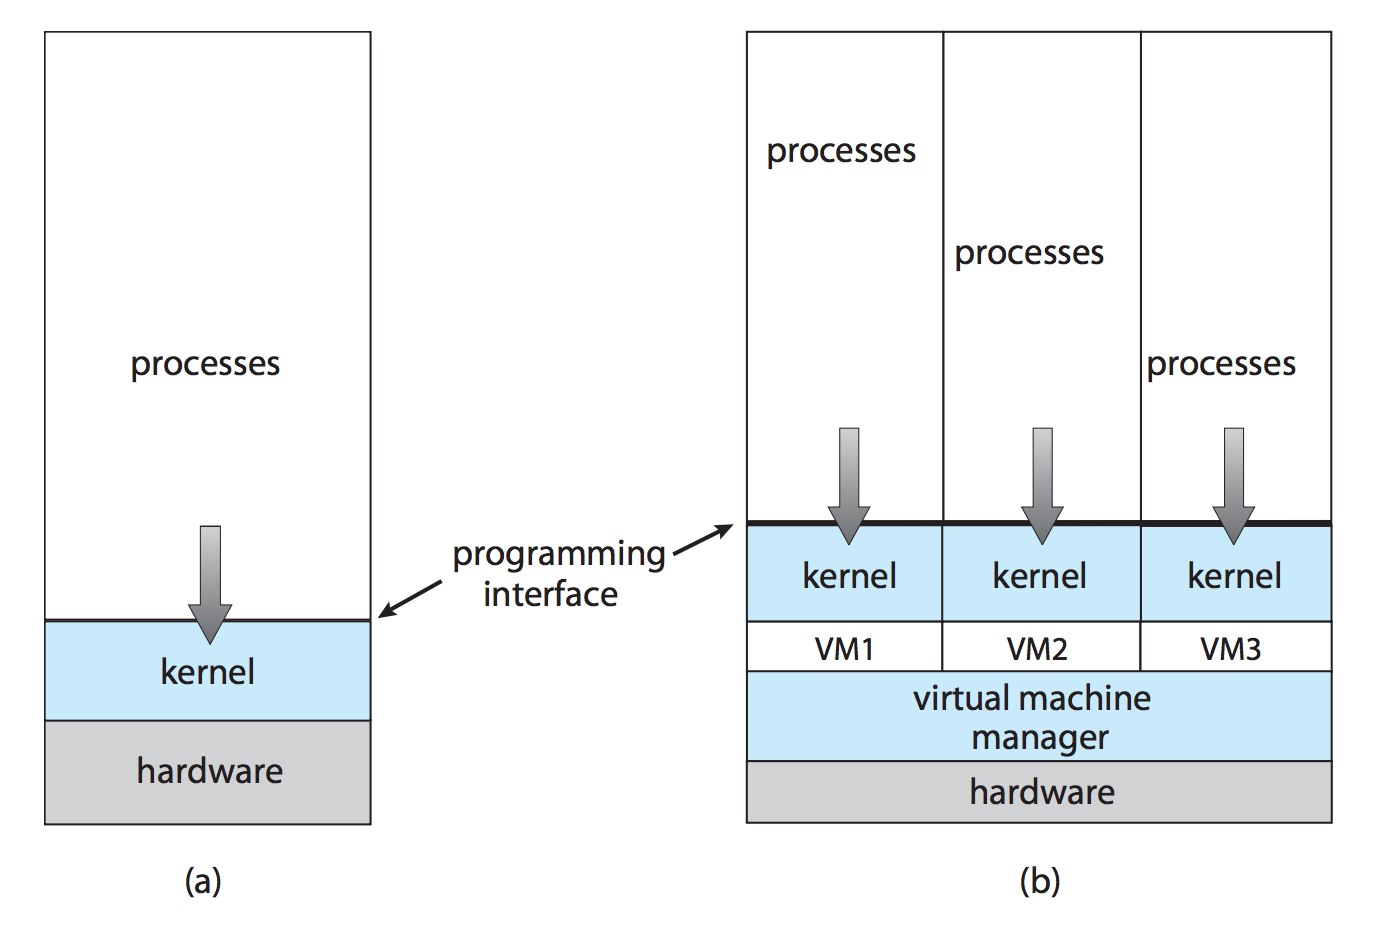
\includegraphics[width=0.6\textwidth]{images/non-virtual-machine.png}\\
	System models: (a) Nonvirtual machine and (b) Virtual machine~\cite{osc}.
\end{center}

This is by no means the same thing as \textit{emulation}. When we have virtualization, for example, both Windows and Linux can be running on the same x86\_64 architecture as guests. In the case of the Android emulator running in an x86\_64 machine, the code of the emulator is running on the x86\_64 environment to simulate an Android hardware device that would have a completely different CPU. Thus, an Android app (which would not otherwise run on an Intel/AMD machine) runs in a simulation of a mobile environment. The emulation operation is incredibly slow, unfortunately, as anyone who has tried to use the Android emulator has found out. Sometimes, however, it does not much matter; if you are trying to play a classic game that ran under MS-DOS, emulating an 486 computer does not take much by way of resources and the modern computer can do so with ease.

Those who run operating systems that are not named ``Microsoft Windows'' are likely to have had the situation where one or more programs that are needed for some purpose (work, school, whatever) function only under Windows. And as the versions of Windows have proliferated and evolved, older programs have sometimes stopped working, necessitating a past version (Windows XP will never, ever die...).

Another neat thing is the ability to suspend (pause) execution of a running virtual machine. This is like pausing a process: the current state is taken and saved, and can be restored at a later time. Also like a process, it can be moved around to another system and resume after that move has taken place, or cloned to get an identical copy somewhere else.

A third reason for virtualization is protection. The guests are isolated from the host and vice versa. If a virus infects one of the guests, the other guests are not affected. And with a virtual machine, it will be that much easier to delete and reinstall the guest or roll it back to an earlier state. This would be exactly the state that we have stored when suspending it... just take periodic copies of it.

Finally, we often see consolidation in data centres: there are many servers running that could be sharing the same physical hardware. Instead of having a lot of lightly used physical systems, convert them to virtual and put them all in the same physical machine. This is often combined with a utility to convert a physical machine to a virtual one; all the system data and configuration and such is copied and turned into a snapshot and this snapshot is then started up inside the virtual machine.

\subsection*{Behind the Scenes}

One of the key building blocks of virtualization is the \textit{virtual CPU} (VCPU). It does not actually execute code; it is just the state of the CPU according to the guest machine. The VMM is responsible for maintaining the state of the VCPU. Much like the process control block, the VCPU is a data structure that is used to store the state when the guest is not running and the state is restored from the VCPU structure when the guest is scheduled to run~\cite{osc}.

Recall from earlier the concept of user mode and kernel mode; application processes run in user mode and the kernel runs in kernel mode, having access to privileged instructions like I/O instructions and poking around with registers and other hardware. The guest operating system runs in user mode, but it will want to do some things that require kernel mode, so we will need to have virtual user mode and virtual kernel mode. Actions like an I/O request or interrupt that would normally lead to a switch from user to kernel mode needs to cause a transfer from virtual user mode to virtual kernel mode.

The first strategy for implementing this is called \textit{trap-and-emulate}. If the guest attempts a privileged instruction, it will generate a trap (error) because it is in user mode. The VMM should then pick this up and executes, emulating (or simulating, if you prefer) the requested operation.

\begin{center}
	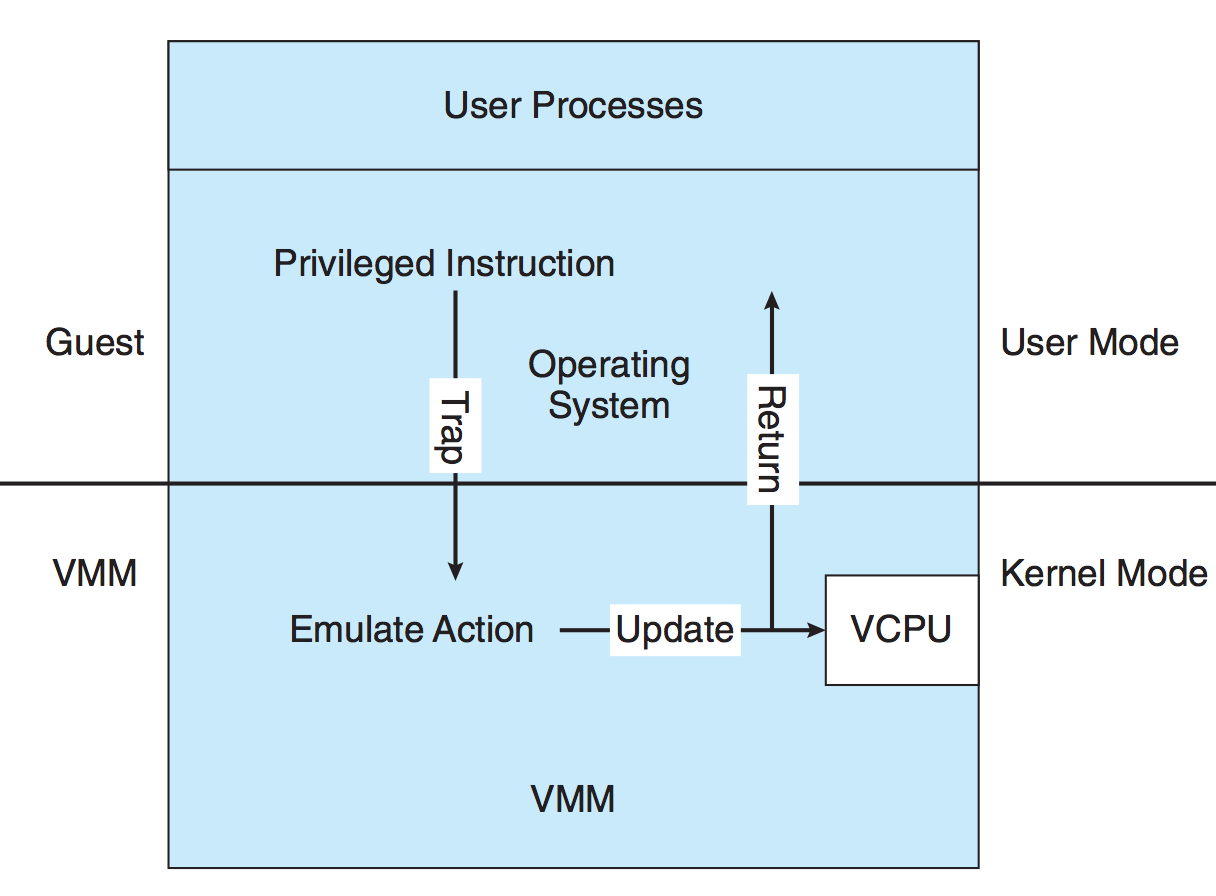
\includegraphics[width=0.5\textwidth]{images/trap-and-emulate.png}\\
	The trap-and-emulate virtualization implementation~\cite{osc}.
\end{center}

Non-privileged instructions just execute natively on the hardware, so they are about as fast as they would be if they were actually being executed outside a virtual machine. Unfortunately, with trap-and-emulate, privileged instructions have this extra overhead, causing the guest to run more slowly than it otherwise would. To get around this problem, hardware designers have come to the rescue again: some CPUs have more than just the two simple modes (user/kernel) and keep track in hardware of virtual user and virtual kernel mode. That relieves the VMM from the responsibility of keeping track of it all in the VCPU~\cite{osc}.

Sadly, some CPUs do not have clear definitions of privileged vs. non-privileged instructions, including the intel x86 architecture (and its descendant, the x86\_64). Without editorializing too much, there were a lot of decisions that went into things like the x86 architecture, C programming language, design of Windows, et cetera, that make no sense if we look at them with what we know today, but they ``seemed like a good idea at the time''. The x86 architecture started back in the early 1970s and we can hardly fault the designers for not anticipating what was going to happen in computing technology 30-40 years later. As a Danish proverb of disputed origin says, ``Making predictions is hard, especially about the future.''

Returning from that small interruption, the x86 has an instruction \texttt{POPF} that illustrates the problem. It loads the flag register from the contents of the stack. If the CPU is in kernel mode, all flags are replaced from the stack; otherwise only some flags are replaced. No trap will be generated if \texttt{POPF} is executed in user mode, so the trap-and-emulate solution will not catch this and react. All instructions that fall into this category are usually referred to as \textit{special instructions} because they require special handling~\cite{osc}.

To get around this problem, we will use a technique called \textit{binary translation}. It is more or less exactly what it sounds like. If the guest VCPU is in user mode, the guest can run its instructions natively. If the guest VCPU is in kernel mode, then the guest believes it is running in kernel mode. The VMM looks at every instruction before they get to the CPU to execute. If they are regular instructions, they can execute natively. If they are special instructions, they are translated into (replaced with) alternative instructions that produce the same result~\cite{osc}.

\begin{center}
	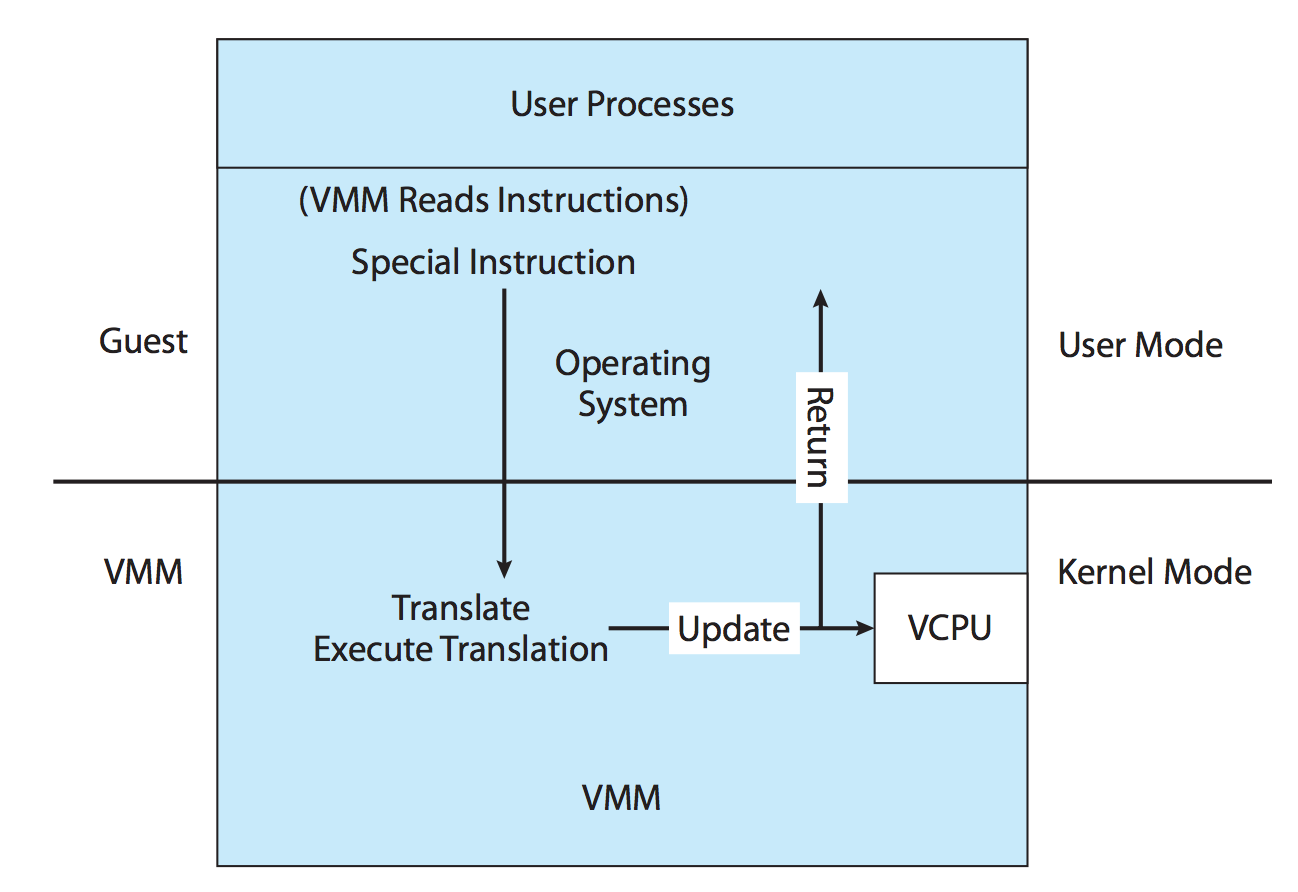
\includegraphics[width=0.5\textwidth]{images/binary-translation.png}\\
	The binary translation virtualization implementation~\cite{osc}.
\end{center}

Although we have a performance decrease as a result of having to examine and replace some of the instructions, most instructions can run natively and only a small number of them need to be emulated. The empirical test of ``what is being used in industry'' seems to indicate that the performance of binary translation is adequate, as there is now widespread adoption of virtual machines running on x86 hardware.

Okay, the last paragraph was a little bit misleading, because additional hardware support has come along to make virtualization work a lot better than it would have. Starting in 2005, Intel added virtualization support to x86 processors and AMD added it in 2006. This breaks down the old rules of dual-mode (kernel/user) processors into multi-mode operation. The VMM can enable host mode, define a guest's characteristics, and then switch to guest mode, passing control to the guest. If the guest tries to access a virtualized resource, the VMM takes over to manage the interaction~\cite{osc}.


\subsection*{The Impact}

The short version of what happens under virtualization is: things get complicated. There are more demands on and difficulties in resources. We will consider the impact on scheduling, memory management, I/O, and disk~\cite{osc}.

\subsubsection*{Scheduling}

Even if there is only one CPU in the physical machine, virtualization presents one or more virtual CPUs to the guests. The challenge then, is to schedule the virtual CPUs' operations on the physical CPU(s). A thread may be a VMM thread or a guest thread.

A guest system is configured with some number of CPUs and as long as there are enough CPUs in the system to meet the allocation commitments (virtual CPU count is less than $n$), we have no problem. Map each virtual CPU to a physical CPU and we are all set. 

If the resources are fully committed (e.g., there are $n$ virtual CPUs allocated), it gets a bit more interesting. The VMM does not (usually) need too much time on its own, so it can basically ``steal'' cycles here and there. VMM operations run on CPUs that are not busy at the moment, or taking evenly from all the CPUs so as to be ``fair''. 

If the situation is overcommitted (there are more virtual CPUs than physical ones), the problem is more interesting. The VMM will have to figure out a way to map the virtual CPUs to the physical ones according to some scheduling strategy. Like scheduling processes and threads, we can use one of the scheduling algorithms we discussed earlier to schedule all of the threads (or at least choose which guest operating system gets to run right now).

When overcommitment is the situation, the expectation of the guest operating system of certain time deadlines becomes inaccurate. If the scheduler in the guest operating system defines a timeslice as, for example, 50~ms, in reality the actual length of a time slice will vary based on how often the VMM chooses to run that guest's threads. It could, in fact, be significantly longer than the 50~ms intended. This is frustrating to the users and has a tendency to get the system clock out of whack, but may be fatal for any real-time operating system or any task with serious wall-clock deadlines.

\subsubsection*{Memory Management}

Virtualization makes the memory problem a lot worse than it otherwise would be. The processes that run take up plenty of memory all on their own, and where we previously had one operating system and its structures in memory, now there are multiple operating systems and their structures taking up memory space, too. The problem is only exacerbated if memory is overcommitted (the amount of memory the guests are allocated exceeds the RAM of the physical machine). There are a few strategies to alleviate the problem, as outlined in~\cite{osc}.

\paragraph{Nested Page Tables.} The guest operating system, unaware it is in a virtual machine, thinks it controls memory and page table management. In reality, the virtual machine manager has a nested page table that re-translates the guest's page  table to the real (physical) page table. The VMM can provide double-paging, where it has its own page replacement strategy and tries to help out the guest. The problem is that the VMM knows less about the guest's memory patterns than the guest itself, so this strategy is inefficient.

\paragraph{Device Driver.} The next idea is then to install, where possible, a device driver into the guest that allows the VMM to exercise some measure of control over the guest. Where the guest OS allows, the device driver from the VMM is installed. When needed, this ``balloon'' memory manager is told to request a whole bunch of (empty) memory and asks the guest to pin its pages in physical memory. This makes the guest think that memory is in short supply and the guest will start to free up memory. The VMM knows that the balloon pages are not real and can allocate them to some other guest. If the memory pressure in the whole system goes down, the balloon pages can be deallocated or unpinned, allowing the guest to feel as if it has more free memory.

\paragraph{Duplicate Detection.} A third idea is for the VMM to look to see if the same page is loaded more than once. This is obviously more likely if the guests are identical (i.e., the same OS). This will result in significant savings, as the operating system may take up a significant portion of memory on its own. To make the operation efficient, a hash value for memory may be taken; if two hashes match then a byte-by-byte comparison will reveal whether they are actually identical. If so, no need to keep both copies in memory. If there is a modification to a shared page, we need to copy the page before the modification is made.

\subsubsection*{Input/Output}
Unlike CPUs and RAM, the guest OSes are likely to tolerate the fact that the I/O devices may change periodically and during operation, such as when a user plugs in a USB key or moves into range of a WiFi network. In fact, we have device drivers as the interface to the OS, regardless of what type of device it is. When running in a virtual machine, a guest may see several virtual devices as if they were real~\cite{osc}.

The VMM can decide how to allocate I/O devices to guests; one way is to just dedicate the I/O device to a guest such as a USB key being allocated to one guest in particular. In other cases, the VMM provides drivers that are just translating commands into the actual device commands. 

\subsubsection*{Disk}

The typical approach is to create a \textit{disk image}, that contains all the contents of the root disk of the guest. This is one big file (though it can be split up into manageable-sized chunks) and as far as the guest is concerned it has the run of that whole disk, totally unaware that the disk is just a file inside another system. This makes it a lot easier to move a virtual machine around from one system to another, if desired.

\section*{Containerize This!}

Containerization gives many of the advantages of this separation of VMs, but without nearly so much overhead of the guest operating systems (both its maintenance and runtime costs). Containers are run by a container engine so there is some abstraction of the underlying hardware, and the container is assembled from a specification that says what libraries, tools, etc. are needed. And thus when the container is built and deployed it is sufficiently isolated but shares (in read only mode) where it can. So a container is a very lightweight VM, in some sense. See this diagram from~\cite{netappcontainer}:

\begin{center}
	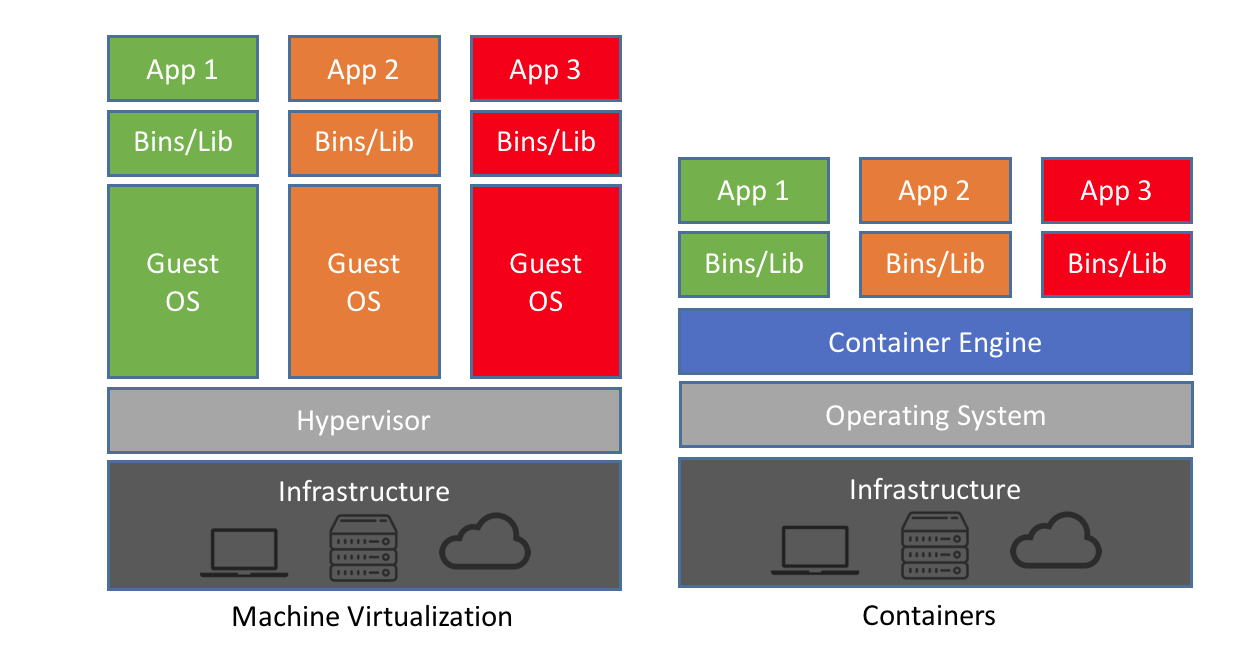
\includegraphics[width=0.55\textwidth]{images/cvm.png}
\end{center}

Containers are a very effecting way of allowing virtualization, but a major potential limitation is that container applications can only run on hosts with the same OS and same virtualization features~\cite{osi}.


\bibliographystyle{alphaurl}
\bibliography{350}


\end{document}